\documentclass[]{article}
\usepackage{graphicx}
\usepackage{float}
\usepackage{hyperref}

%opening
\title{Renovation of Harman Kardon 430 Twin}
\author{George Biro}

\begin{document}

\maketitle

\begin{abstract}
This work presents the restoration and performance evaluation of a Harman Kardon 430 Twin receiver. The unit was refurbished by replacing known failure-prone semiconductor devices and aging passive components, followed by verification of operating points across all major circuit blocks.

Comprehensive electrical measurements were carried out to assess the performance of the phono and auxiliary (AUX) input stages. Frequency-domain analysis based on high-resolution FFT techniques was used to evaluate total harmonic distortion (THD), signal-to-noise ratio (SNR), and intermodulation distortion (IMD) over a wide frequency range.

The results show that the restored unit achieves low distortion levels, with the AUX input demonstrating superior performance due to its simpler signal path and lower gain. The phono stage exhibits slightly higher noise and distortion, as expected from its equalization and amplification requirements, but remains within acceptable limits for high-fidelity reproduction.

Overall, the measurements confirm that the restoration successfully returns the receiver to stable and reliable operation, with performance characteristics consistent with its original design.

\end{abstract}

\section{Introduction}

The unit was purchased for 200\,EUR plus shipping.  
Initially, it was operational; however, sound quality exhibited noticeable distortion and noise artifacts.
All switches and potentiometers were cleaned using Tesanol 26026 contact cleaner.

\section{Disclaimer}

This document is provided for informational purposes only. While every effort has been made to ensure the accuracy and completeness of the information contained herein, the author assumes no responsibility or liability for any errors, omissions, or inaccuracies.

All modifications, repairs, and measurements described in this document are performed at the reader's own risk. The author shall not be held liable for any damage to equipment, property, or personal injury resulting from the use or application of the information provided.

All replacement components were tested prior to installation; however, no warranty, express or implied, is given regarding their performance, reliability, or suitability for any particular purpose.

\section{Measurement and Test Equipment}

\begin{table}[H]
	\centering
	\caption{Measurement and Test Equipment Used}
	\label{tab:tools}
	\begin{tabular}{ll}
		\hline
		\textbf{Instrument Type} & \textbf{Model} \\
		\hline
		AD Converter & E1DA COSMOS ADC ISO Grade B (ES9822Pro, 32-bit, 768\,kHz) \\
		LCR Meter & DER EE DE-5000 \\
		Line-Phono Converter & OMNITRONIC LH-042 \\
		Multimeter & UNI-T UT980C \\
		Oscilloscope & Hameg HM303-4 \\
		Signal Generator & UNI-T UTG932E \\
		VA/Ohm Meter & Philips PM2503 \\
        Transistor Tester & Peak Atlas DCA55 \\
		\hline
	\end{tabular}
\end{table}

Frequency-domain analysis was performed using a custom FFT processing framework developed by the author (\textit{Yet Another Audio Analyzer, YAAR}) \cite{yaar}.


\section{Power Supply Boards}

\begin{table}[H]
	\centering
	\caption{Power Supply Repair Log}
	\label{tab:power_supply_log}
	\begin{tabular}{|l|l|l|}
		\hline
		\textbf{Ref.} & \textbf{Original} & \textbf{Replacement} \\
        \hline
        C1,C15 & $1000\,\mu\mathrm{F} / 35\,\mathrm{V}$ & A758BG106M1EAAE070 \\
        \hline
        C2,C4 & $2200\,\mu\mathrm{F} / 35\,\mathrm{V}$ & A758EK226M1EAAE050 \\
        \hline
        C3 & $470\,\mu\mathrm{F} / 25\,\mathrm{V}$ & EEU-FC2A2R2H \\
        \hline
        C6,C7,C8,C9 & $4700\,\mu\mathrm{F} / 35\,\mathrm{V}$ & retained \\
        \hline
        D5 & SIB01-02 & 1N4007 (Vishay) \\
        \hline
        D6 & IS 2372A & B380C1000G-E4/51 \\
        \hline
        Q1, Q2 & 2SC1212C & BD139-16 (STmicro, $h_{FE} \approx 135$) \\
        \hline
	\end{tabular}
\end{table}

Modern $4700\,\mu\mathrm{F} / 35\,\mathrm{V}$ capacitors are significantly smaller in size and would not match the original visual appearance. As the existing capacitors showed no signs of leakage or external damage and performed within specification, they were retained.

\begin{table}[H]
	\centering
	\caption{Rectifier Voltages}
	\label{tab:rectifier_voltages}
	\begin{tabular}{|l|l|l|l|}
		\hline
		\textbf{Ref.} & \textbf{B} & \textbf{C} & \textbf{E} \\
    \hline
    Q1 &  12.83V & 30.4V  &   12.16V \\
    \hline
    Q2 &  25.6V & 29.99V &  24.95V \\
    \hline
	\end{tabular}
\end{table}

\begin{table}[H]
	\centering
	\caption{Power Supply Voltages}
	\label{tab:power_suppy_volt}
	\begin{tabular}{|l|l|}
		\hline
		\textbf{Ref.} & \textbf{V} \\
        \hline
        LP3-LP4 & 45.6VAC \\
        \hline
        LP5-LP6 & 45.6VAC \\
        \hline
        B1+ &  +30.55V (120mV ripple) \\
        \hline
        B1- &  -30.59  (120mV ripple) \\
        \hline
        B2+ &  +30.55V (120mV ripple) \\
        \hline
        B2- &  -30.55V (120mV ripple) \\
        \hline
        B3+ & 12.16V \\
        \hline
        B4+ & 24.95V \\
        \hline
	\end{tabular}
\end{table}

\section{Equalizer Amp}

Due to the known reliability issues associated with the 2SC1344 transistors, all devices of this type were replaced with KSC1845F equivalents.

\begin{table}[H]
	\centering
	\caption{Equalizer Amp Repair Log}
	\label{tab:eq_amp_log}
	\begin{tabular}{|l|l|l|}
		\hline
		\textbf{Ref.} & \textbf{Original} & \textbf{Replacement} \\
		\hline
		Q701,Q702,Q703,Q704 & 2SC1344E & KSC1845F (onsemi, $h_{FE} \approx 450$) \\
        \hline
        C701,C702 & 10uF/16V & A758BG106M1EAAE070 \\
        \hline
        C705,C706 & 47uF/6.3V & EEU-FS2A470L \\
        \hline
        C711,C712 & 0.47uF/35V & R82EC3470AA70J \\
        \hline
        C717,C718 & 100uF/25V & EEU-FR1V101B \\
        \hline
	\end{tabular}
\end{table}


\begin{table}[H]
	\centering
	\caption{Equalizer Amp Voltages}
	\label{tab:eq_amp_voltages}
	\begin{tabular}{|l|l|l|l|}
    \hline
 \textbf{Ref.} & \textbf{B} & \textbf{C} & \textbf{E} \\
    \hline
    Q701 & 590mV  & 1.678  & 31.9mV   \\
    \hline
    Q702 & 595mV  & 1.688  & 35mV   \\
    \hline
    Q703 & 1.67  & 8.5  &  1.04  \\
    \hline
    Q704 & 1.68  & 10.35  & 1.03   \\
    \hline
	\end{tabular}
\end{table}

\section{Tone/Pre Amp Board}

Due to the known reliability issues associated with the 2SC1344 transistors, all devices of this type were replaced with KSC1845F equivalents.

\begin{table}[H]
	\centering
	\caption{Tone/Pre Amp Repair Log}
	\label{tab:tone_amp_log}
	\begin{tabular}{|l|l|l|}
		\hline
		\textbf{Ref.} & \textbf{Original} & \textbf{Replacement} \\
		\hline
		Q501,Q502,Q503,Q504,Q505,Q506 & 2SC1344E & KSC1845F (onsemi, $h_{FE} \approx 450$) \\
        \hline
        C503,C504 & 10uF/16V & A758BG106M1EAAE070 \\
        \hline
        C505,C506 & 22uF/10V & A758EK226M1EAAE050 \\
        \hline
        C513,C514 & 2.2uF/50V & EEU-FC2A2R2H \\
        \hline
        C517,C518 & 47uF/16V & A750EK476M1EAAE040 \\
        \hline
	\end{tabular}
\end{table}

\begin{table}[H]
	\centering
	\caption{Tone/Pre Amp Voltages}
	\label{tab:tone_amp_voltages}
	\begin{tabular}{|l|l|l|l|}
    \hline
 \textbf{Ref.} & \textbf{B} & \textbf{C} & \textbf{E} \\
    \hline
    Q501 & 4.11V & 24.95V &   3.55V  \\
    \hline
    Q502 & 4.20V & 24.95V  &   3.61V  \\
    \hline
    Q503 & 604mV & 5.75V  &  33.7mV  \\
    \hline
    Q504 & 603mV & 5.82V &  32.9mV  \\
    \hline
    Q505 & 5.79V & 24.88V  & 5.23V \\
    \hline
    Q506 & 5.86V & 24.91V  &  5.27V \\
    \hline
	\end{tabular}
\end{table}

\section{Main Amp Board}

Due to the well-known reliability issues associated with the 2SC1345F transistors, all devices of this type were replaced with KSC1845F equivalents.

Several 2SC1509R and 2SA777 transistors exhibited a current gain ($h_{FE}$) below 60, which was considered indicative of degradation or failure. These devices were therefore replaced with high-quality modern equivalents (TTC004B.Q and TTA004B.Q).

The 2SC458 transistors, which are also known for poor long-term reliability, were likewise replaced with KSC1845F devices.

No direct modern equivalent for the 2SC1030C is available. The device was not removed from the circuit; however, in-circuit measurements indicated normal operation, and it was therefore retained.

\begin{table}[H]
	\centering
	\caption{Main Amp Repair Log}
	\label{tab:main_amp_log}
	\begin{tabular}{|l|l|l|}
		\hline
		\textbf{Ref.} & \textbf{Original} & \textbf{Replacement} \\
		\hline
		Q401,Q402,Q403,Q404,Q405,Q406 & 2SC1345F & KSC1845F (onsemi, $h_{FE} \approx 450$) \\
        \hline
        Q407,Q408,Q415,Q116 & 2SC1509R & TTC004B.Q (Toshiba, $h_{FE} \approx$ 180) \\
        \hline
        Q409,Q410,Q413,Q414 & 2SA777R & TTA004B.Q (Toshiba, $h_{FE} \approx$ 180)\\
        \hline
        Q421,Q422 & 2SC458B & KSC1845F (onsemi, $h_{FE} \approx 450$)\\
        \hline
        C401,C402 & $47\,\mu\mathrm{F} / 16\,\mathrm{V}$ & R82EC3470AA70J  \\
        \hline
        C404,C405 & $220\,\mu\mathrm{F} / 16\,\mathrm{V}$  & A758KK227M1CAAE014 \\
        \hline
        C407,C408 & $1000\,\mu\mathrm{F} / 16\,\mathrm{V}$ & EEU-FS1H102L \\
        \hline
        D401,D402,D403,D404,D405,D406 & 1S2076 & 1N4148 (onsemi) \\
        \hline
        D407,D408 & SIB01-02 & 1N4007 (Vishay) \\
        \hline
	\end{tabular}
\end{table}

\begin{table}[H]
	\centering
	\caption{Main Amp Voltages}
	\label{tab:main_amp_voltages}
	\begin{tabular}{|l|l|l|l|}
    \hline
 \textbf{Ref.} & \textbf{B} & \textbf{C} & \textbf{E} \\
    \hline
    Q401 & -66.8mV  & 29.48V  & -0.682V   \\
    \hline
    Q402 & -68.3mV  & 29.9V  & -0.675V   \\
    \hline
    Q403 & -58.2mV  & 30.05V  &  -0.67V  \\
    \hline
    Q404 & -65.3mV & 29.9V &  -0.67V   \\
    \hline
    Q405 & -28.7V  & -0.66V & -29.3V   \\
    \hline
    Q406 & -28.9V  & -0.65V  & -29.3V    \\
    \hline
    Q407 & -29.6V  &  -0.72V &  -30.2V  \\
    \hline
    Q408 & -29.6V  &  -0.72V & -30.2V   \\
    \hline
    Q409 & 30.2V  &  1.22V &  29.6V  \\
    \hline
    Q410 & 30.2V  &  1.22V &  29.7V  \\
    \hline
    Q421 & -57mV  & 1.22V  &  -0.75V  \\
    \hline
    Q422 & -54mV  & 1.25V  & -0.74V   \\
    \hline
    Q413 & -149mV  & -30.06V  &   -0.72V \\
    \hline
    Q414 & -160mV  & -30.07V  &  -0.73V  \\
    \hline
    Q415 & 1.24V  & 30.5V  &  0.65V  \\
    \hline
    Q416 & 1.25V  & 30.5V  & 0.66V    \\
    \hline
    Q417 &  0.65V & 30.5V  & 42mV   \\
    \hline
    Q418 & 0.66V  & 30.5V & 45mV   \\
    \hline
    Q419 & -29.99V  & -10mV & -30.6V \\
    \hline
    Q420 & -29.99V & -10mV & -30.6V \\
    \hline
	\end{tabular}
\end{table}

\section{Tuner Section}

The FM and AM tuner boards were not modified during the restoration. Functional testing confirmed that radio reception operates correctly, with stable tuning and good signal quality. Basic measurements did not reveal any abnormalities, indicating that the tuner section is operating within specification.

\section{Final Measurements}

All output voltage and power measurements (e.g., 10\,V\textsubscript{rms} reference levels) were verified using a calibrated Philips PM2503 VA/Ohm meter, as listed in the measurement equipment. The voltage and power values shown in the FFT plots generated by the audio analyzer are dependent on the configuration of the ADC (e.g., input range and DIP switch settings) and should therefore be considered indicative only. Consequently, absolute amplitude values reported by the FFT framework were not used for quantitative evaluation.

\subsection{Phono Stage}

The signal generator was set to an output level of 450\,mV\textsubscript{rms} and connected to the input of the inverse RIAA converter. The output of the converter was fed into the phono input of the amplifier. An 8\,\(\Omega\) load resistor was connected to the amplifier output, and the volume control was adjusted to obtain an output power of approximately 12.5\,W. The same input voltage and volume setting were maintained for all test frequencies.

The measured spectra show a consistent harmonic structure across all test frequencies. At low frequencies (56\,Hz and 243\,Hz), the distortion is dominated by low-order harmonics (primarily 2nd and 3rd), with THD values around 0.04--0.05\%. At these frequencies, the noise floor is relatively elevated, resulting in higher THD+N values (up to approximately 0.6\%). This indicates that the measurement is partially noise-limited rather than purely distortion-limited.

In the mid-frequency range (987\,Hz), the distortion remains low and stable, with THD around 0.04--0.06\%, suggesting proper linear operation of the equalizer and gain stages.

At higher frequencies (6.999\,kHz and 14.997\,kHz), a slight increase in THD is observed, particularly on the right channel where values approach 0.09\%. This behavior is typical and can be attributed to bandwidth limitations and increased nonlinearity in the amplifier stages at higher frequencies.

A small but consistent channel imbalance is visible, with the right channel generally exhibiting slightly higher distortion and lower SNR compared to the left channel. This may indicate minor component tolerances or residual mismatch in the signal path.

The IMD measurements (CCIF test at 18.987\,kHz and 20.001\,kHz) show very low intermodulation products, with SMPTE IMD around 0.14\% and no significant CCIF artifacts. This confirms good high-frequency linearity and absence of severe slew-rate or crossover-related distortion.

Overall, the phono stage demonstrates good linearity and expected performance for a vintage design, with distortion remaining below 0.1\% across the measured frequency range.

\begin{figure}[H]
	\centering
	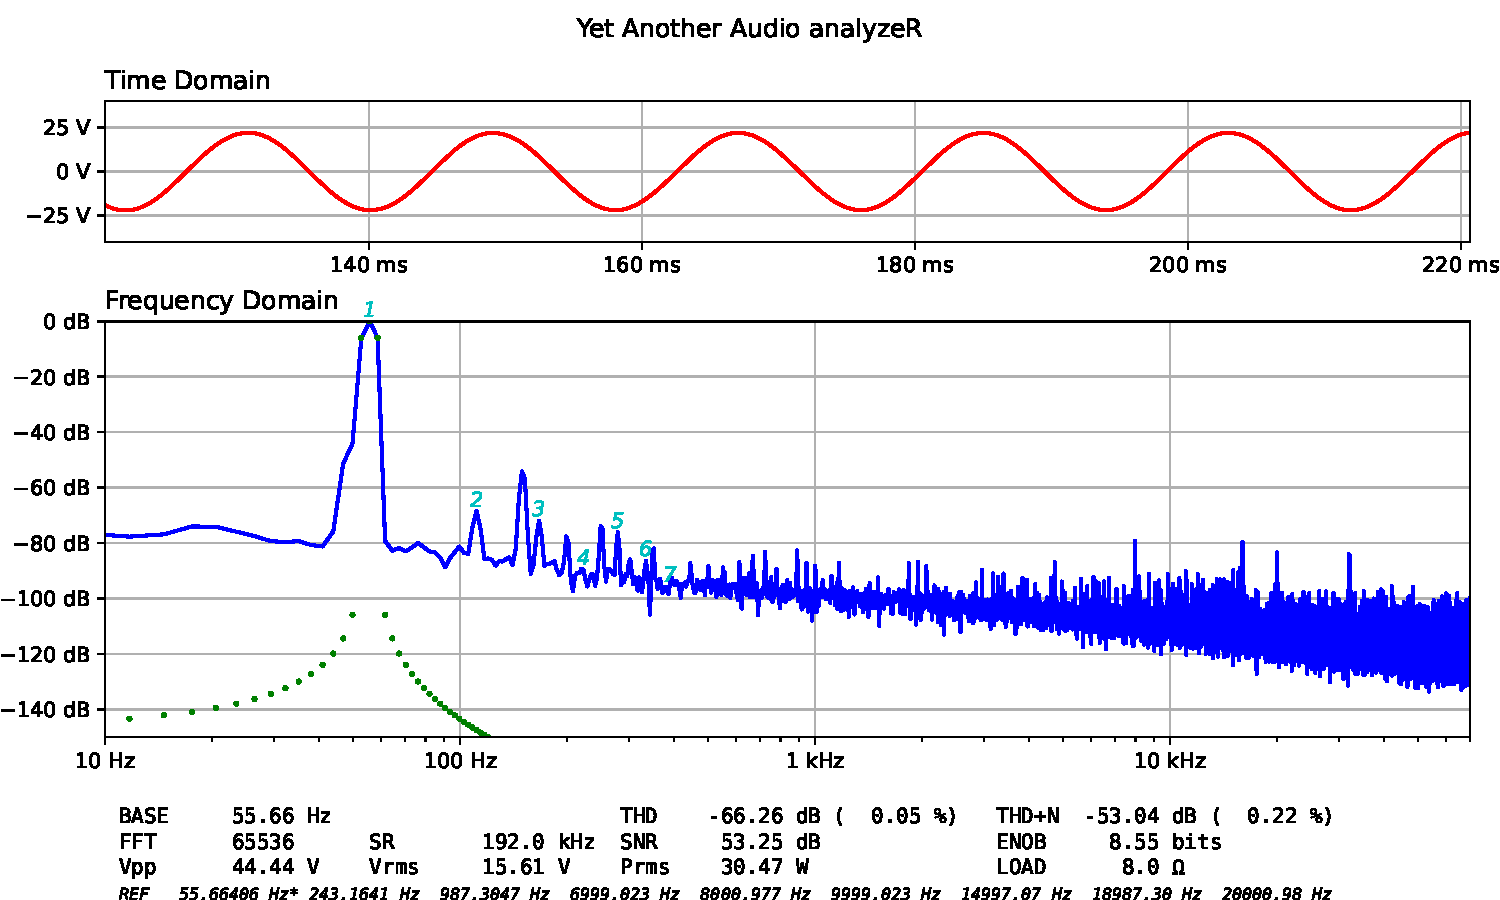
\includegraphics[width=\linewidth]{measurements/hk430_phono_left_56Hz_0Hz.pdf}
	\caption{THD measurement of the left phono channel at 56\,Hz}
	\label{fig:phono_56Hz_left}
\end{figure}

\begin{figure}[H]
	\centering
	
\includegraphics[width=\linewidth]{measurements/hk430_phono_left_243Hz_0Hz.pdf}
	\caption{THD measurement of the left phono channel at 243\,Hz}
	\label{fig:phono_243Hz_left}
\end{figure}

\begin{figure}[H]
	\centering
	
\includegraphics[width=\linewidth]{measurements/hk430_phono_left_987Hz_0Hz.pdf}
	\caption{THD measurement of the left phono channel at 987\,Hz}
	\label{fig:phono_987Hz_left}
\end{figure}

\begin{figure}[H]
	\centering
	
\includegraphics[width=\linewidth]{measurements/hk430_phono_left_6999Hz_0Hz.pdf}
	\caption{THD measurement of the left phono channel at 6\,999\,Hz}
	\label{fig:phono_6999Hz_left}
\end{figure}

\begin{figure}[H]
	\centering
	
\includegraphics[width=\linewidth]{measurements/hk430_phono_left_14997Hz_0Hz.pdf}
	\caption{THD measurement of the left phono channel at 14\,997\,Hz}
	\label{fig:phono_14997Hz_left}
\end{figure}

\begin{figure}[H]
	\centering
	
\includegraphics[width=\linewidth]{measurements/hk430_phono_right_56Hz_0Hz.pdf}
	\caption{THD measurement of the right phono channel at 56\,Hz}
	\label{fig:phono_56Hz_right}
\end{figure}

\begin{figure}[H]
	\centering
	
\includegraphics[width=\linewidth]{measurements/hk430_phono_right_243Hz_0Hz.pdf}
	\caption{THD measurement of the right phono channel at 243\,Hz}
	\label{fig:phono_243Hz_right}
\end{figure}

\begin{figure}[H]
	\centering
	
\includegraphics[width=\linewidth]{measurements/hk430_phono_right_987Hz_0Hz.pdf}
	\caption{THD measurement of the right phono channel at 987\,Hz}
	\label{fig:phono_987Hz_right}
\end{figure}

\begin{figure}[H]
	\centering
	
\includegraphics[width=\linewidth]{measurements/hk430_phono_right_6999Hz_0Hz.pdf}
	\caption{THD measurement of the right phono channel at 6\,999\,Hz}
	\label{fig:phono_6999Hz_right}
\end{figure}

\begin{figure}[H]
	\centering
	
\includegraphics[width=\linewidth]{measurements/hk430_phono_right_14997Hz_0Hz.pdf}
	\caption{THD measurement of the right phono channel at 14\,997\,Hz}
	\label{fig:phono_14997Hz_right}
\end{figure}

\begin{figure}[H]
	\centering
	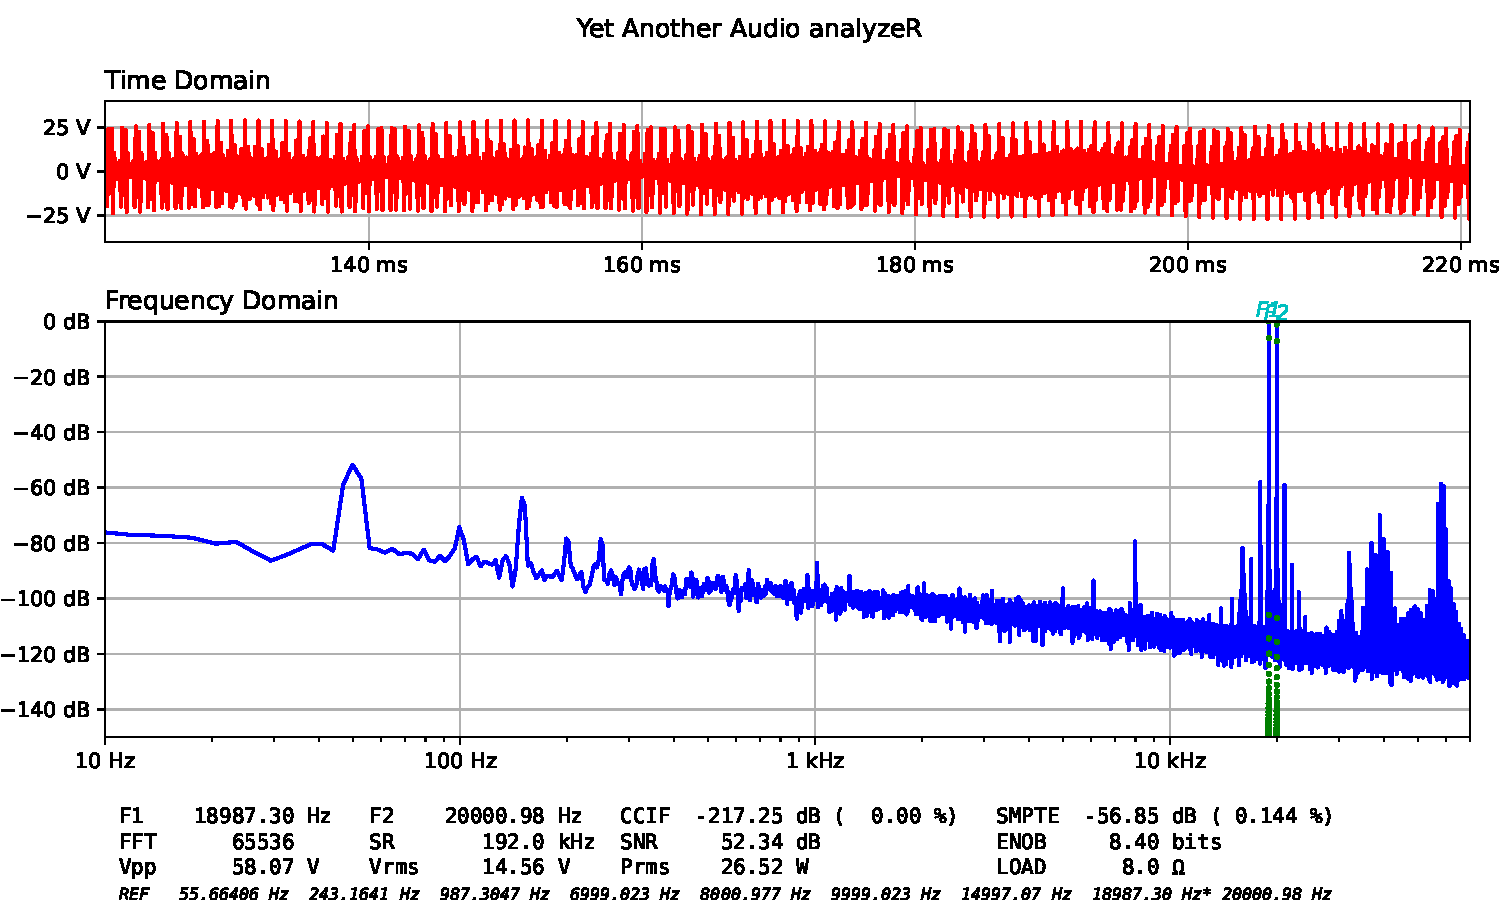
\includegraphics[width=\linewidth]{measurements/hk430_phono_left_imd_18987Hz_20001Hz.pdf}
	\caption{IMD measurement of the left phono channel (18\,987\,Hz and 20\,001\,Hz)}
	\label{fig:phono_18987Hz_20001Hz_left}
\end{figure}

\begin{figure}[H]
	\centering
	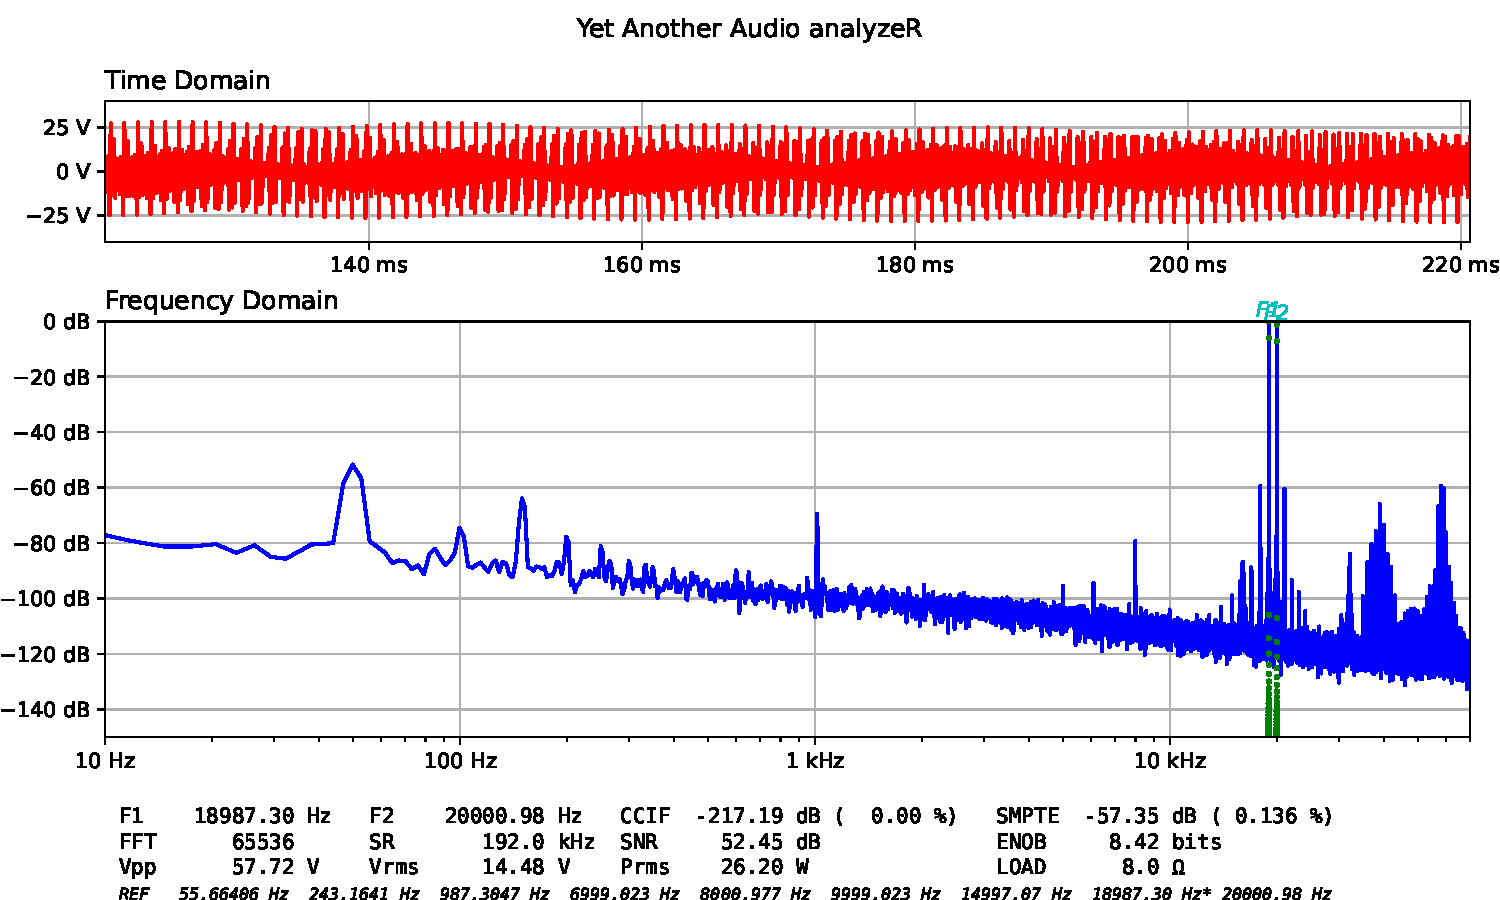
\includegraphics[width=\linewidth]{measurements/hk430_phono_right_imd_18987Hz_20001Hz.pdf}
	\caption{IMD measurement of the right phono channel (18\,987\,Hz and 20\,001\,Hz)}
	\label{fig:phono_18987Hz_20001Hz_right}
\end{figure}

\subsection{Aux}

The signal generator was set to an output level of 250\,mV\textsubscript{rms} and connected to the AUX1 input of the amplifier. An 8\,\(\Omega\) load resistor was connected to the amplifier output, and the volume control was adjusted to obtain an output power of approximately 25\,W. The same input voltage and volume setting were maintained for all test frequencies.

The AUX input measurements show significantly improved performance compared to the phono stage, as expected due to the absence of RIAA equalization and lower overall gain.

Across all test frequencies, the spectra are clean with a well-defined fundamental and low harmonic content. THD values remain in the range of approximately 0.03--0.05\%, with THD+N closely matching THD, indicating that the measurements are distortion-limited rather than noise-limited.

The noise floor is substantially lower than in the phono measurements, resulting in improved SNR (up to approximately 70\,dB) and higher effective resolution. This reflects the simpler signal path and reduced amplification requirements of the AUX input stage.

No significant increase in distortion is observed at higher frequencies (up to 14.997\,kHz), suggesting adequate bandwidth and stable operation of the preamplifier and power amplifier stages under these conditions.

The harmonic structure is dominated by low-order components, with higher-order harmonics remaining well suppressed. Channel matching is generally good, with only minor deviations between left and right channels.

Overall, the AUX input exhibits clean and stable performance with low distortion, confirming proper operation of the line-level signal path after restoration.

The IMD measurements for the AUX input were performed using a CCIF test signal consisting of two closely spaced high-frequency tones at 18\,987\,Hz and 20\,001\,Hz. The resulting spectra show well-defined fundamentals with minimal intermodulation products in the baseband region.

The CCIF intermodulation components are effectively suppressed, with no significant difference-frequency products visible above the noise floor. The SMPTE IMD values remain low, indicating good linearity of the amplification stages even under high-frequency two-tone excitation.

Compared to the phono stage, the AUX input exhibits a cleaner spectrum with a lower noise floor and reduced spurious components. This is expected due to the simpler signal path and absence of high-gain equalization stages.

No signs of slew-rate limiting or high-frequency instability are observed, as evidenced by the absence of elevated sidebands around the fundamental tones. The symmetric distribution of any residual components suggests predominantly low-order nonlinearities.

Overall, the AUX IMD performance is excellent, confirming that the line-level signal path operates with high linearity and minimal intermodulation distortion across the tested frequency range.

\begin{figure}[H]
	\centering
	
\includegraphics[width=\linewidth]{measurements/hk430_aux_left_56Hz_0Hz.pdf}
	\caption{THD measurement of the left AUX channel at 56\,Hz}
	\label{fig:aux_56Hz_left}
\end{figure}

\begin{figure}[H]
	\centering
	
\includegraphics[width=\linewidth]{measurements/hk430_aux_left_243Hz_0Hz.pdf}
	\caption{THD measurement of the left AUX channel at 243\,Hz}
	\label{fig:aux_243Hz_left}
\end{figure}

\begin{figure}[H]
	\centering
	
\includegraphics[width=\linewidth]{measurements/hk430_aux_left_987Hz_0Hz.pdf}
	\caption{THD measurement of the left AUX channel at 987\,Hz}
	\label{fig:aux_987Hz_left}
\end{figure}

\begin{figure}[H]
	\centering
	
\includegraphics[width=\linewidth]{measurements/hk430_aux_left_6999Hz_0Hz.pdf}
	\caption{THD measurement of the left AUX channel at 6\,999\,Hz}
	\label{fig:aux_6999Hz_left}
\end{figure}

\begin{figure}[H]
	\centering
	
\includegraphics[width=\linewidth]{measurements/hk430_aux_left_14997Hz_0Hz.pdf}
	\caption{THD measurement of the left AUX channel at 14\,997\,Hz}
	\label{fig:aux_14997Hz_left}
\end{figure}

\begin{figure}[H]
	\centering
	
\includegraphics[width=\linewidth]{measurements/hk430_aux_right_56Hz_0Hz.pdf}
	\caption{THD measurement of the right AUX channel at 56\,Hz}
	\label{fig:aux_56Hz_right}
\end{figure}

\begin{figure}[H]
	\centering
	
\includegraphics[width=\linewidth]{measurements/hk430_aux_right_243Hz_0Hz.pdf}
	\caption{THD measurement of the right AUX channel at 243\,Hz}
	\label{fig:aux_243Hz_right}
\end{figure}

\begin{figure}[H]
	\centering
	
\includegraphics[width=\linewidth]{measurements/hk430_aux_right_987Hz_0Hz.pdf}
	\caption{THD measurement of the right AUX channel at 987\,Hz}
	\label{fig:aux_987Hz_right}
\end{figure}

\begin{figure}[H]
	\centering
	
\includegraphics[width=\linewidth]{measurements/hk430_aux_right_6999Hz_0Hz.pdf}
	\caption{THD measurement of the right AUX channel at 6\,999\,Hz}
	\label{fig:aux_6999Hz_right}
\end{figure}

\begin{figure}[H]
	\centering
	
\includegraphics[width=\linewidth]{measurements/hk430_aux_right_14997Hz_0Hz.pdf}
	\caption{THD measurement of the right AUX channel at 14\,997\,Hz}
	\label{fig:aux_14997Hz_right}
\end{figure}

\begin{figure}[H]
	\centering
	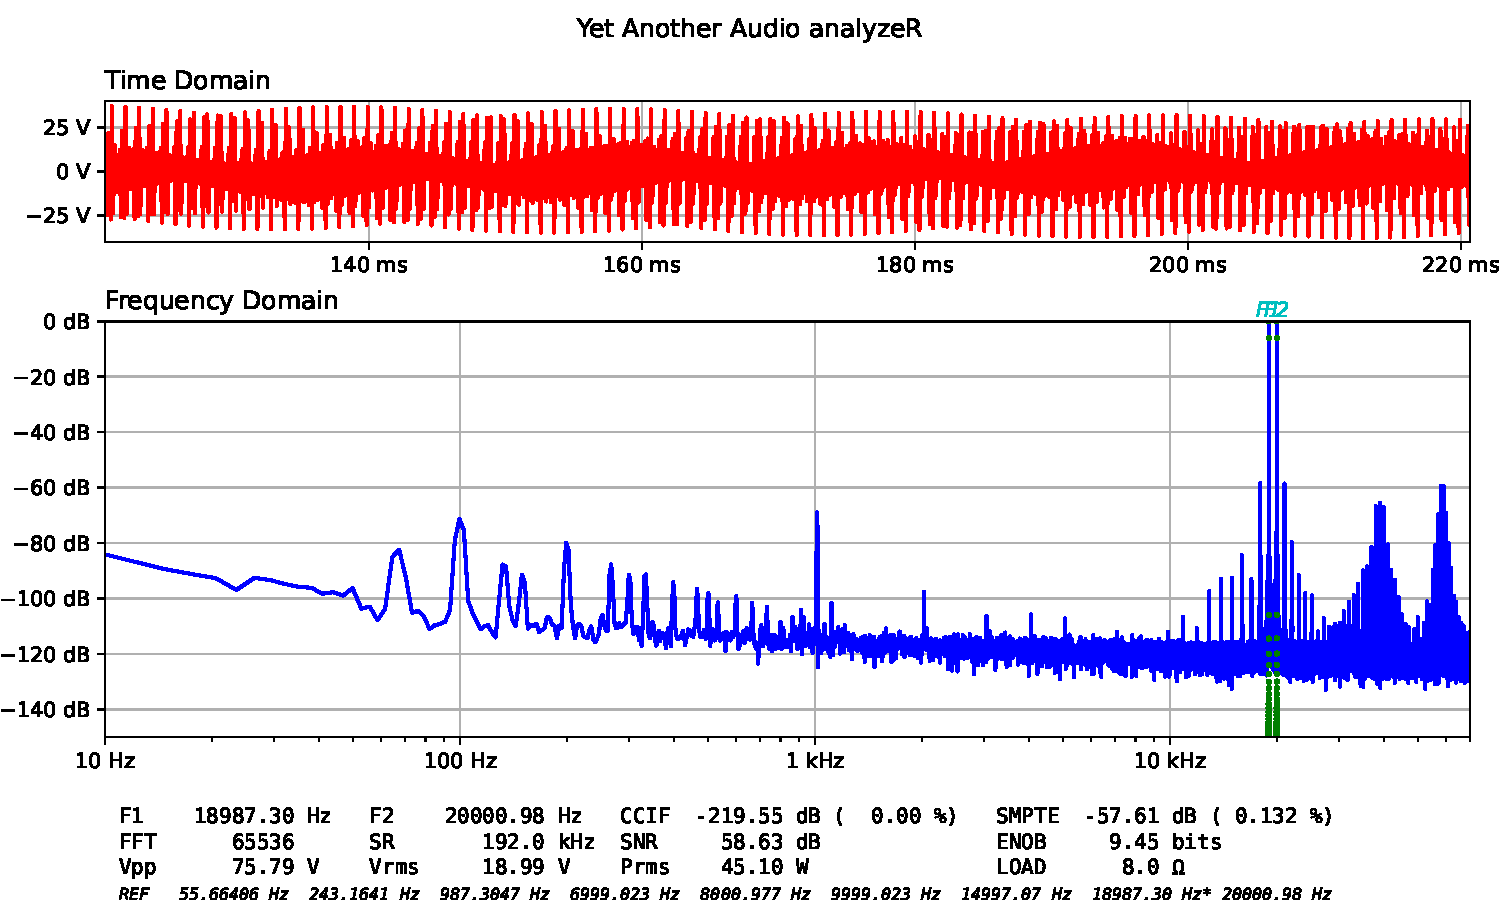
\includegraphics[width=\linewidth]{measurements/hk430_aux_left_imd_18987Hz_20001Hz.pdf}
	\caption{IMD measurement of the left AUX channel (18\,987\,Hz and 20\,001\,Hz)}
	\label{fig:aux_18987Hz_20001Hz_left}
\end{figure}

\begin{figure}[H]
	\centering
	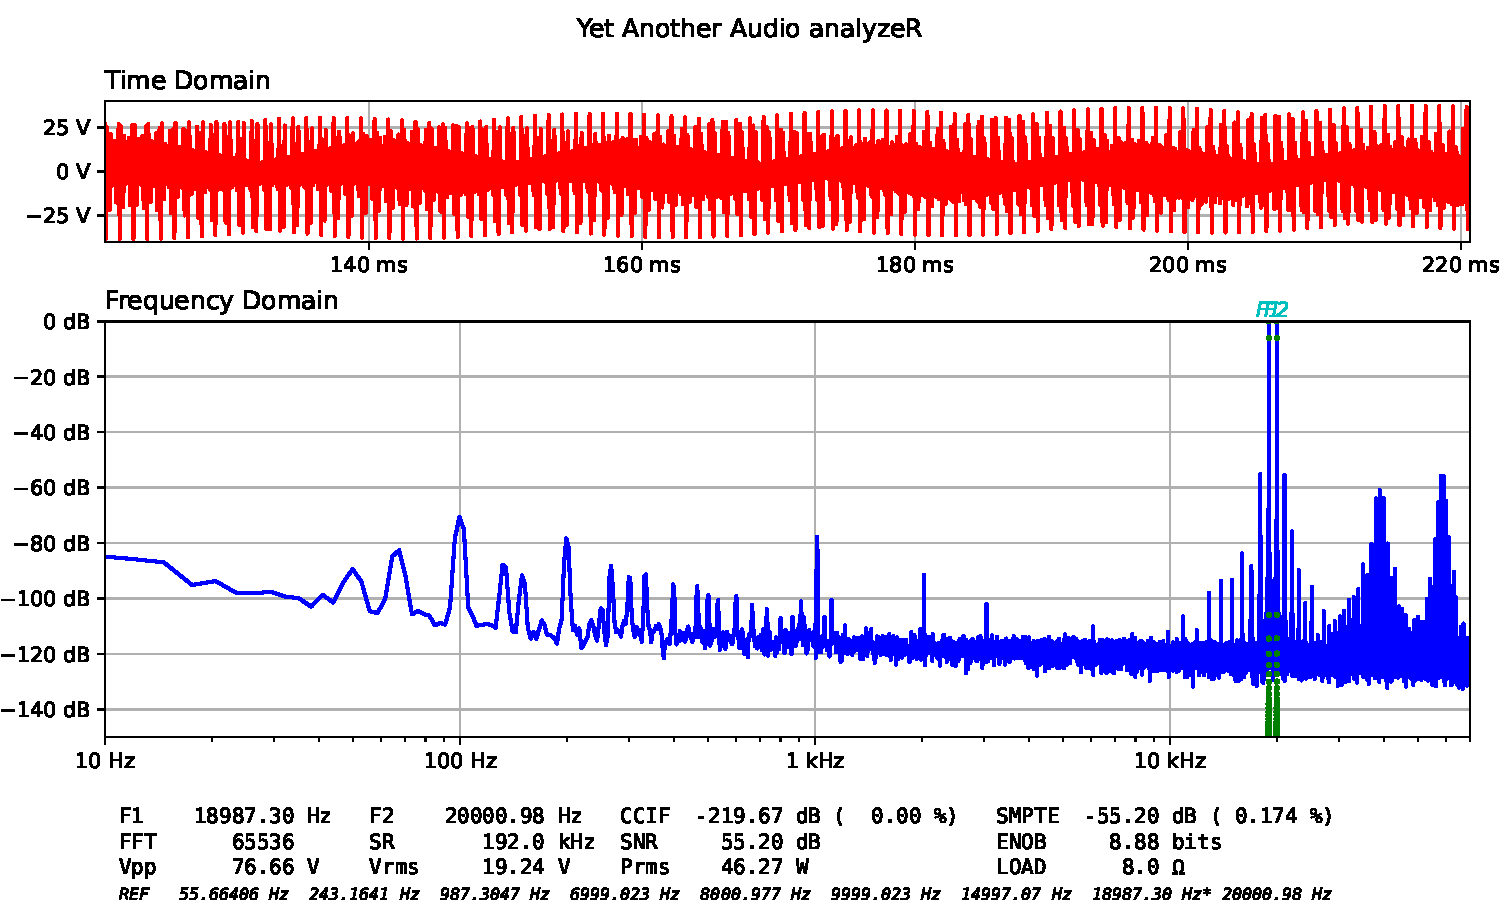
\includegraphics[width=\linewidth]{measurements/hk430_aux_right_imd_18987Hz_20001Hz.pdf}
	\caption{IMD measurement of the right AUX channel (18\,987\,Hz and 20\,001\,Hz)}
	\label{fig:aux_18987Hz_20001Hz_right}
\end{figure}

\section{Listening Test}

A subjective listening evaluation was conducted to complement the electrical measurements. The restored receiver was tested using both analog and digital program material.

For analog playback, the \textit{Eric Clapton -- Just One Night} LP was used via the phono input. The phono stage delivered a balanced and natural sound, with good clarity in vocals and instruments. Background noise was present at a low level, as expected for a phono stage, but did not interfere with the listening experience. The tonal balance was perceived as warm and consistent with typical characteristics of vintage audio equipment.

For digital playback, a FiiO BTR3 Bluetooth receiver was used as a source, streaming high-resolution audio including recordings by \textit{Bob Dylan}. The AUX input exhibited clean and detailed reproduction, with improved transparency and lower noise compared to the phono input. Dynamic range and stereo imaging were perceived as stable and well-defined.

The system was evaluated using Canton Karat 300 loudspeakers. The combination provided a pleasant listening experience, with sufficient output power, controlled bass response, and clear midrange reproduction. No audible distortion or instability was detected during normal listening levels.

Overall, the listening test confirms the objective measurement results. The AUX input offers superior clarity and lower noise, while the phono stage provides a slightly warmer but still well-controlled sound. The restored receiver performs reliably and delivers enjoyable audio quality in practical use.

The subjective impressions are consistent with the measured performance, particularly the lower noise floor and distortion observed on the AUX input compared to the phono stage.

\section{Conclusion}

The restoration of the Harman Kardon 430 Twin receiver was successful both electrically and functionally. Replacement of known unreliable semiconductor devices and aged capacitors resulted in stable operating points across all circuit stages.

Measurement results confirm good overall performance. The AUX input demonstrates low distortion (typically below 0.05\%) and high signal-to-noise ratio, indicating a clean and linear signal path. The phono stage, while exhibiting higher noise and distortion due to its high gain and equalization requirements, remains within expected limits for vintage equipment, with THD generally below 0.1\%.

A slight channel imbalance was observed, with the right channel showing marginally higher distortion at higher frequencies. However, this does not significantly impact overall performance.

Intermodulation distortion measurements confirm good linearity, with no evidence of slew-rate limiting or instability.

In summary, the restored unit performs in accordance with its original design expectations and is suitable for high-quality audio reproduction.

\begin{thebibliography}{9}

\bibitem{yaar}
G.~Biro, \textit{Yet Another Audio Analyzer (YAAR)}, GitHub repository. Available: \url{https://github.com/george-biro/yet-another-audio-analyzer}

\end{thebibliography}

\end{document}
